\documentclass[11pt]{article}
\usepackage{amsmath,amsbsy,amssymb,verbatim,fullpage,ifthen,graphicx,bm,amsfonts,amsthm,url}
\usepackage{graphicx}
\usepackage{xcolor}
\newcommand{\mfile}[1]  {{\small \verbatiminput{./#1}}} % Jeff Fessler, input matlab file
\newcommand{\tmop}[1]{\ensuremath{\operatorname{#1}}}
\newcommand{\R}{\mathbb{R}}
\newcommand{\C}{\mathbb{C}}
\newcommand{\Z}{\mathbb{Z}}
\newcommand{\A}{\mathcal{A}}
\newcommand{\minimize}{\operatorname*{minimize\ }}
\newcommand{\maximize}{\operatorname*{maximize}}
\newcommand{\opdet}[1]{\operatorname{\textbf{det}}\left(#1\right)}
\newcommand{\optr}[1]{\operatorname{\textbf{tr}}\left(#1\right)}
\newcommand{\answer}[2][blue]{\ifdefined\AnswerDefine{\color{#1}\it#2}\fi}
\newcommand{\mtx}[1]{\mathbf{#1}}
\newcommand{\vct}[1]{\mathbf{#1}}
\def \lg       {\langle}
\def \rg       {\rangle}
\def \mA {\mtx{A}}
\def \mI {\mtx{I}}
\def \mJ {\mtx{J}}
\def \mU {\mtx{U}}
\def \mS {\mtx{S}}
\def \mV {\mtx{V}}
\def \mW {\mtx{W}}
\def \mLambda {\mtx{\Lambda}}
\def \mSigma {\mtx{\Sigma}}
\def \mX {\mtx{X}}
\def \mY {\mtx{Y}}
\def \mZ {\mtx{Z}}
\def \zero     {\mathbf{0}}
\def \vzero    {\vct{0}}
\def \vone    {\vct{1}}
\def \vu {\vct{u}}
\def \vv {\vct{v}}
\def \vx {\vct{x}}
\def \vy {\vct{y}}
\def \vz {\vct{z}}
\def \vphi {\vct{\phi}}
\def \vmu {\vct{\mu}}
\def \R {\mathbb{R}}


\usepackage{xspace}
\makeatletter
\DeclareRobustCommand\onedot{\futurelet\@let@token\@onedot}
\def\@onedot{\ifx\@let@token.\else.\null\fi\xspace}

\def\eg{\emph{e.g}\onedot} \def\Eg{\emph{E.g}\onedot}
\def\ie{\emph{i.e}\onedot} \def\Ie{\emph{I.e}\onedot}
\def\cf{\emph{c.f}\onedot} \def\Cf{\emph{C.f}\onedot}
\def\etc{\emph{etc}\onedot} \def\vs{\emph{vs}\onedot}
\def\wrt{w.r.t\onedot} \def\dof{d.o.f\onedot}
\def\etal{\emph{et al}\onedot} \def\st{\emph{s.t}\onedot}
\pagestyle{plain}

\title{{\bf Homework Set 2, CPSC 8420, Spring 2022}} % Change to the appropriate homework number
\author{\Large{Song, Zhiyuan}}
% put your name in the LastName, FirstName format
\date{\today}

\begin{document}
	\maketitle
	\section*{A. to P1}
	In the case of $\maximize \|\mX \bm{\phi}\|^2_2, \st \ \|\bm{\phi}\|_2=1$,	we can apply te equation\\
	\begin{align}
	\|\mA\|^2_2 = \text{Trace}(\mA^{T}\mA) = \text{Trace}(\mA^T\mA)
	\end{align}
	Consequently, $\maximize \|\mX \bm{\phi}\|^2_2, \st \ \|\bm{\phi}\|_2=1$ is equivalent to
	\begin{align*}
	\maximize \text{Trace}(\bm{\phi}^T\mX^T\mX\bm{\phi}) \st \ \|\bm{\phi}\|_2=1
	\end{align*}
	If we consider an eigen value problem
	\begin{align*}
	\mX^T\mX\bm{\phi}=\lambda\bm{\phi}
	\end{align*}
	Where $\lambda$ is the eigenvalue of $\mX^T\mX$. wW will get to
	\begin{align*}
	\bm{\phi}^T\mX^T\mX\bm{\phi}=\lambda\bm{\phi}=\bm{\phi}^T\lambda\bm{\phi}\equiv\lambda\|\bm{\phi}\|_2=\lambda
	\end{align*}
	Therefore, if we want to maximize the $\bm{\phi}^T\mX^T\mX\bm{\phi}$, it is equivalent to maximize the eigenvalue of $\mX^T\mX$. Accordingly, if we take SVD on $\mX^T\mX$, we will get singular values of $\mX^T\mX$ in order laying on $\mS$ diagnoally as well as $\mU$, where $[\mU,\mS]=svd(\mX^T\mX)$. It will result in the largest $\lambda$ at $\mS_{11}$ and the corresponding eigenvector $\bm{\phi}_1$, which is the first column of $\mU$.
	We can demostrate it using matrix notation. Assume $\left[\mU,\mSigma\right]=\text{SVD}\left(\mX^T\mX\right)$, we will have $\mX^T\mX=\mU\mSigma\mU^T$. Consider an element at the i$^{th}$ row and the j$^{th}$ column of an matrix $\mU$
	\begin{align*}
	\left(\mU\right)_{ij}=u_{ij}
	\end{align*}
	Furthermore, we can denote matrix multiplication, transpose, unitarity and singular value decomposition as
	\begin{gather*}
	\left(\mtx{C}\right)_{ij}=\left(\mA\mtx{B}\right)_{ij}=\sum_{k}a_{ik}b_{kj} \\
	\left(\mA^T\right)_{ij}=a_{ji}\\
	\left(\mA^T\mA\right)=\mI\equiv\sum_{k}\left(\mA^T\right)_{ik}a_{kj}=\sum_{k}a_{ki}a_{kj}=\delta_{ij}\\
	\left(\mSigma\right)_{ij}=\lambda_{i}\delta_{ij}
	\end{gather*}
	Therefore,
	\begin{align*}
	\left(\mX^T\mX\right)_{ij}=\left(\mU\mSigma\mU^T\right)_{ij}=\sum_{m,l}u_{im}\lambda_{m}\delta_{ml}u_{jl}
	\end{align*}
	If we consider to use q$^{th}$ column of $\mU$, $(\bm{\phi}_{q})_{i}=u_{iq}$, and get the corresponding eignvalue, we will have to evaluate
	\begin{align*}
	\bm{\phi}_q^T\left(\mU\mSigma\mU^T\right)\bm{\phi}_q\equiv \\
	\sum_{i}u_{iq}\left(\sum_{m,l}u_{im}\lambda_{m}\delta_{ml}u_{jl}\right)\sum_{j}u_{jq}&=\sum_{m,l}\lambda_{m}\delta_{ml}\overbrace{\sum_{i}u_{im}u_{iq}}^{\delta{mq}}\overbrace{\sum_{j}u_{jl}u_{jq}}^{\delta_{lq}}\\
	&=\lambda_q
	\end{align*}
	As a result, if we want the maximum ($q=1$) singular value of $\mX^T\mX$, we can just calculate $\bm{\phi}_1^T\mX^T\mX\bm{\phi}_1$ in order to $\maximize \|\mX \bm{\phi}\|^2_2, \st \ \|\bm{\phi}\|_2=1$. Moreover, we can consider to use a linear combination of eigenvectors $\mX^T\mX$, $\bm{\psi}$,to act on $\mX^T\mX$
	\begin{align*}
	\bm{\psi}&=\sum_{i}p_i\bm{\phi}_i \ \st \sum_{i}p_i^2=1\\
	\|\bm{\psi}\|_2 & \equiv
	\sum_{k,a}p_a p_k \overbrace{\sum_{i}u_{ia}u_{ik}}^{\delta_{ak}}\\
	&=\sum_{a}p_a p_a=1
	\end{align*}
	\begin{align*}
	\therefore \bm{\psi}_q^T\left(\mU\mSigma\mU^T\right)\bm{\psi}_q\equiv\\
	\sum_{i,k}p_k u_{ik} \left(\sum_{m,l}u_{im}\lambda_{m}\delta_{ml}u_{jl}\right) \sum_{a,j}p_a u_{ja}&=\sum_{m,l,k,a}\lambda_m\delta_{ml}p_k\overbrace{\sum_{i}u_{ik}u_{im}}^{\delta_{km}}p_a\overbrace{\sum_{j}u_{jl}u_{ja}}^{\delta_{la}}\\
	&=\sum_{m}p_m p_m\lambda_m\\
	&\leq \sum_{m}p_m p_m\lambda_{1}=\lambda_1
	\end{align*}
	Therefore, the first column of $\mU$ will be the most optimal eigenvector to get the largest $\lambda$.
	\section*{A. to P2}
	If the dataset includes outlayers, the sum of square residuals may amply such differences, leaading to biased centroids. Different from $K$-means, $K$-medians update a centroid by calculating the median value of data points inside the cluster. Besides, $k$-medians will be evaluated by summation of absolute residuals. Here is a specific experiment to present their different as shown in Figure \ref{fig:p1}. Centroids in $K$-median clusters showed less impact from added outlyers than $K$-means. Besides, they performed differently on iterations and clustering results as well as different objective scores. 
	\begin{figure}
		\centering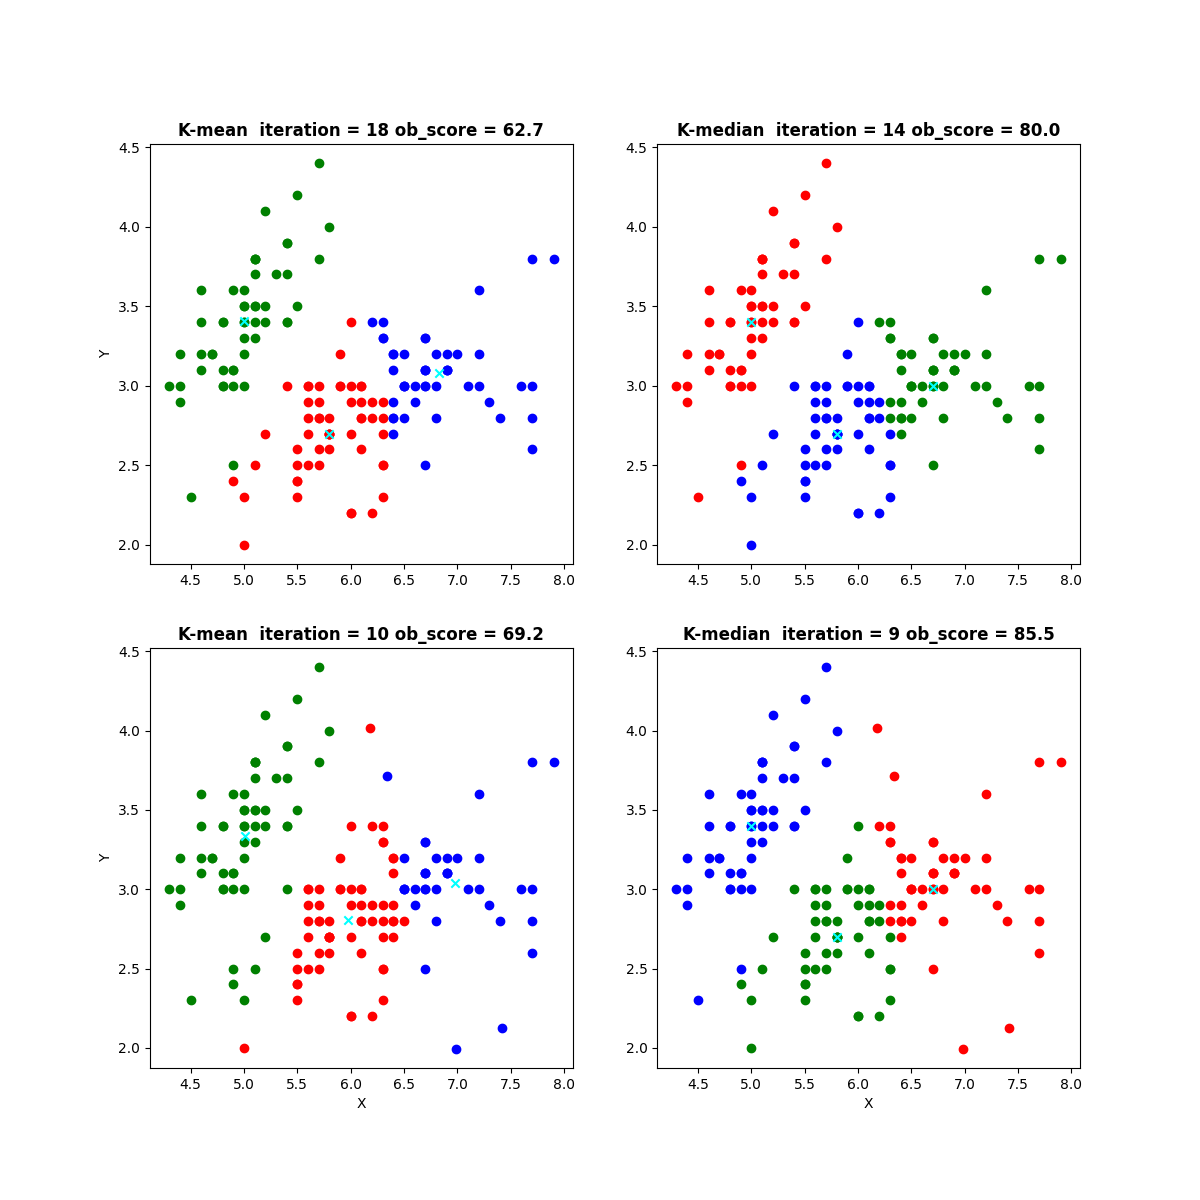
\includegraphics[width=.75\linewidth]{prob2.png}
		\caption{\textbf{Differences of $K$-means and $K$-medians on clustering the same datapoints} Upper two pannels shows the clustering results without outlayers. While lower two include outlayers. Green, blue red denote different clusters; Cyan points denote centroids of the corresponding clusters. } % caption of the figure
		\label{fig:p1}  % Label the figure so you can refer to it in text.
	\end{figure}
	\mfile{class_used_prob2.py}
	\section*{A. to P3}
	\begin{enumerate}
		\item
		If we take SVD on the matrix $\mA \in \R^{n\times p}$, we can get $\mA=\left[\mU\mSigma\mV^T\right]$, where $\mU \in \R^{n\times n}$, $\mSigma \in \R^{n\times n}$, and $\mV\in\R^{p\times n}$, instead of $\mU \in \R^{n\times p}$, $\mSigma \in \R^{p\times p}$, and $\mV\in\R^{p\times p}$. Then, we can calculate $\mA^T=\mV\mSigma\mU^T$. Therefore,
		\begin{align*}
		\mA^T\mA&=\mV\mSigma\mU^T\mU\mSigma\mV^T\\
		&=\mV\mSigma^2\mV^T\\
		\end{align*}
		Consider that
		\begin{align*}
		\left(\mA\mtx{B}\mtx{C}\right)^{-1}=\mtx{C}^{-1}\mtx{B}^{-1}\mA^{-1}
		\end{align*}
		We should have obtained
		\begin{align*}
		\left(\mA^T\mA\right)^{-1}&=\left(\mV\mSigma^2\mV^T\right)\\
		&=\left(\mV^T\right)^{-1}\left(\mSigma\right)^{-2}\left(\mV\right)^{-1}
		\end{align*}
		However, neither $\mV \in \R^{p\times n}$ nor $\mV^T \in \R^{n \times p}$, is invertible. Therefore, in the case of $\mA \in\R^{n\times p}$ and $p>n$, $\mA^T\mA$ is not invertible, leading to the inapplicable $(\mA^T\mA)^{-1}\mA^T\vy$.
		
		\item \& 3.
		The form of ridge regression will reduce to general least square form as well as the learning rate form if $\lambda$ is set to be zero. Hence, sub-problem 2 and 3 can be taken together into account such that $\lambda$ varies from $0,0.1,1,10,100,200$. Normalized objective scores were computed to emphasize the converge of the gradient descent method. Otherwise, the scores would change too slightly to see the decreases. Besides, the precison was set to be $10^{-5}$ on percent difference instead. As shown in Figure \ref{fig:p2}, the learning and convergence rates decreased when $\lambda$ increased, suggesting faster converges and shorter iterations.
		\begin{figure}
			\centering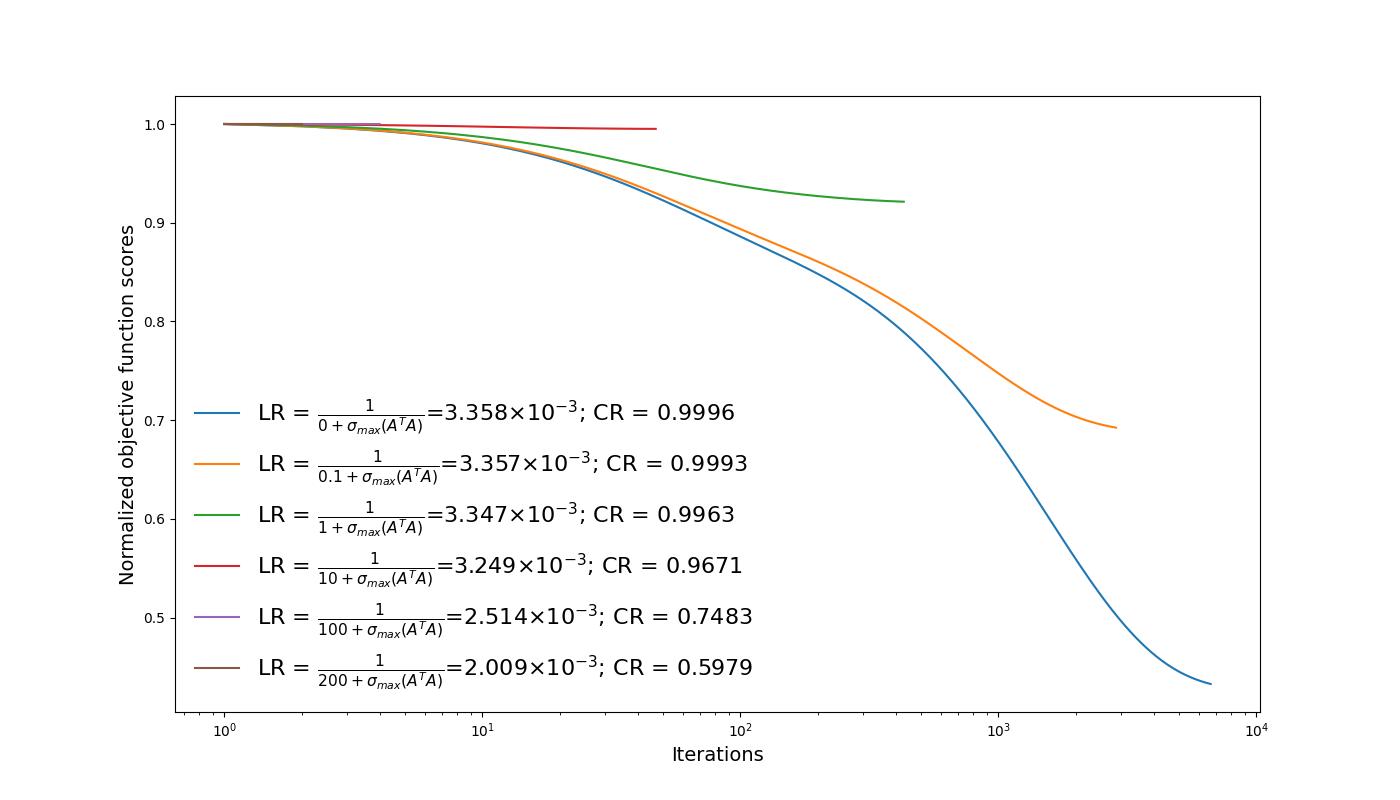
\includegraphics[width=.75\linewidth]{prob3.png}
			\caption{ \textbf{Normalized objective function scores vs iteration steps in logspace} The learning rate for each $\lambda$ was denoted as LR and convergence rates were denoted as CR} % caption of the figure
			\label{fig:p2}
		\end{figure}
	\mfile{prob3-fix.py}
	\end{enumerate}
	\section*{A. to P4}
	Figure \ref{fig:p3} shows the reconstructed images with the corresponding principal components. As the principal number increases, the resolution of the image becomes higher. The way I defined to determine the number of principal numbers is to consider both the cumulative variance of the reconstructed image matrix to the original one and the number of principal components. The equivalent objective funtion
	\begin{align*}
	\sum_{i,j}^{m,n}\left(a_{ij}-z_{ij}\right)^2+k
	\end{align*}
	Where $a_{ij}$ denote the reconstructed image matrix, $z_{ij}$ refers to the original matrix, and $k$ is the number of selected principal components. However, the variance-like term and component term were normalized to their maximum calculation in practice, which is to keep the same order of magnitude for two terms, as shown in \ref{fig:p4}. Therefore, the best trade-off in my case will be around 42 principal components. The outcome image will be better than the one involving 20 components but vaguer than the one involving 50 components in Figure \ref{fig:p3}.
	\begin{figure}
		\centering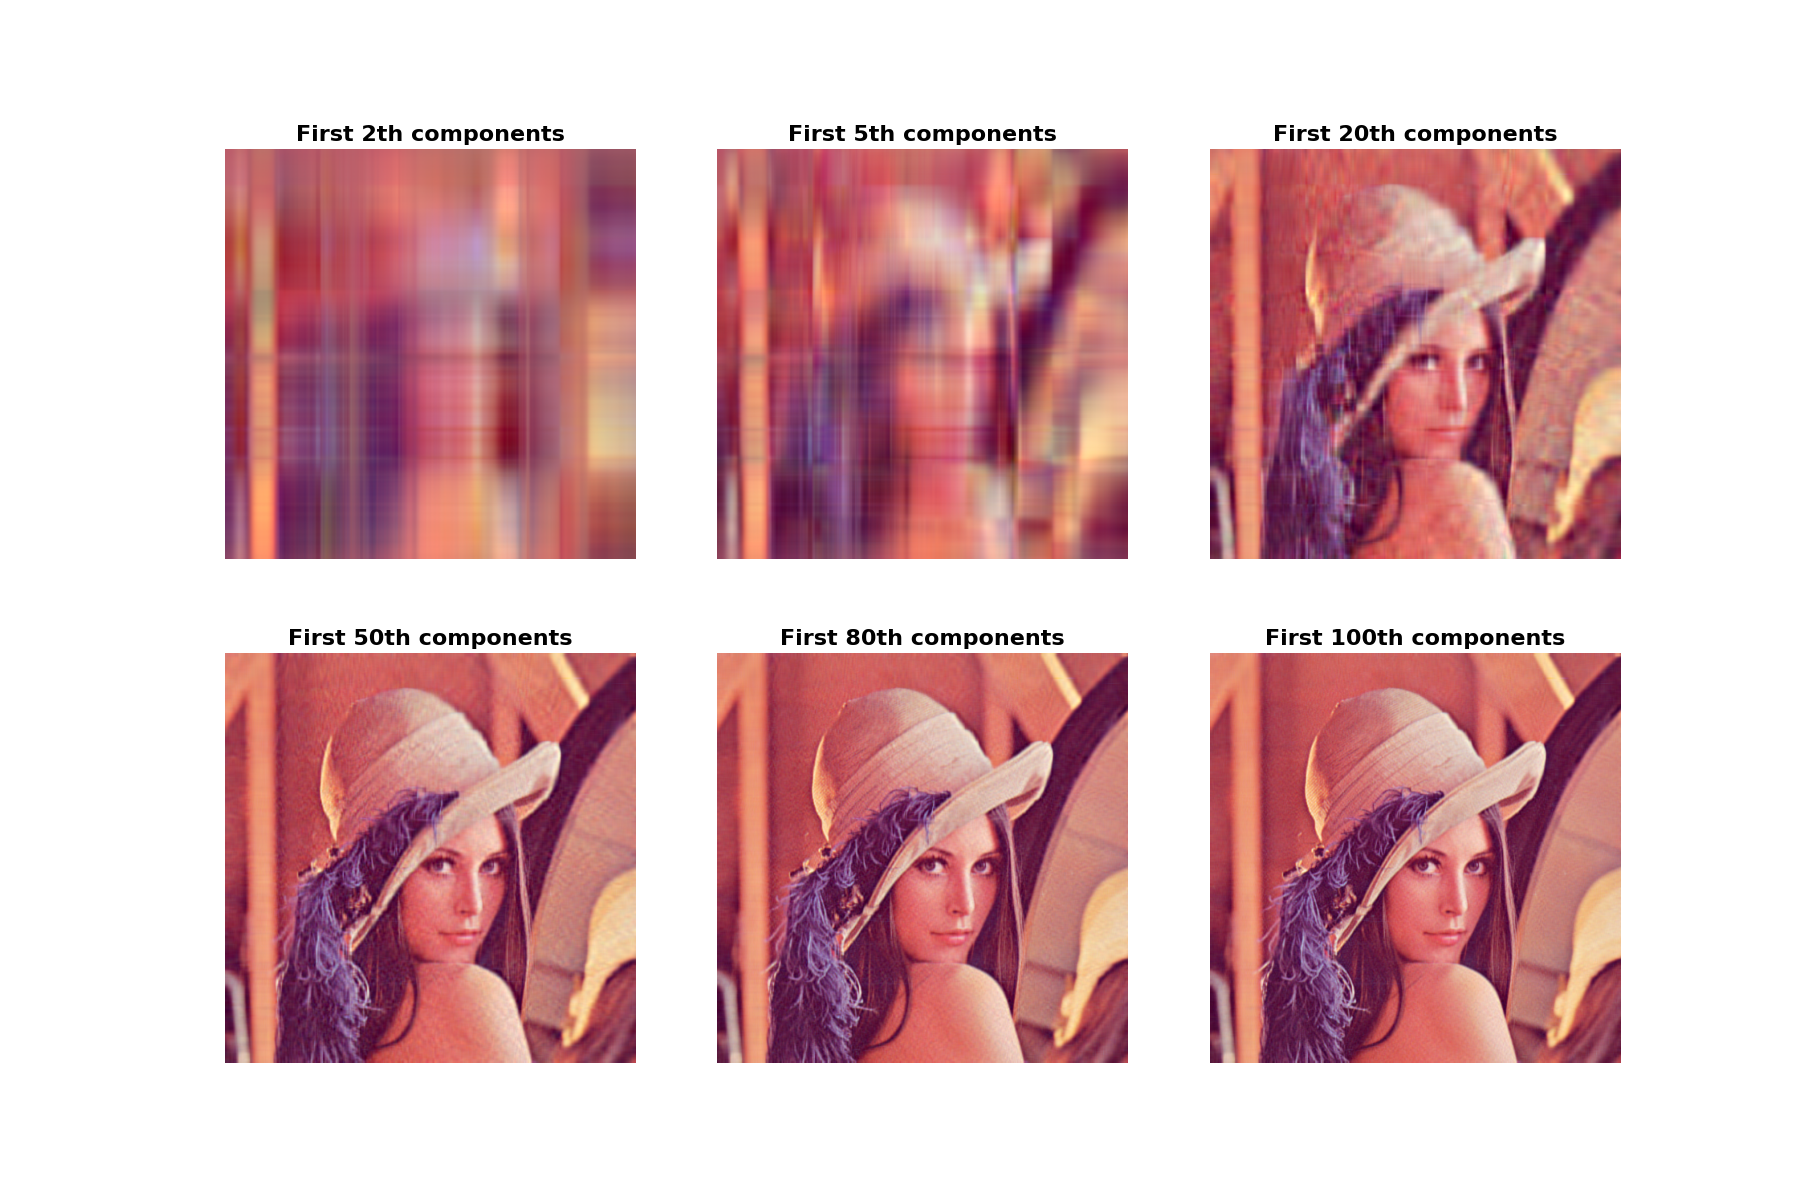
\includegraphics[width=.75\linewidth]{prob4.png}
		\caption{ \bf Image reconstructions with the increase of the size of the eigenvector set} % caption of the figure
		\label{fig:p3}
	\end{figure}
	\mfile{prob4.py}
	\begin{figure}
		\centering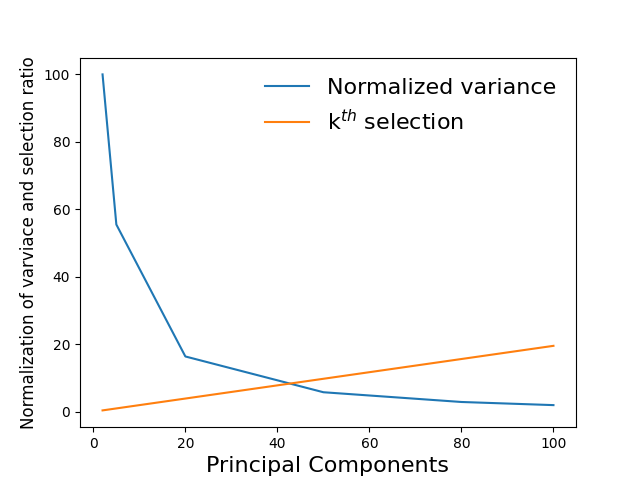
\includegraphics[width=.75\linewidth]{prob4-2.png}
		\caption{ \bf Normalized cumulative variace and the number of principal component} % caption of the figure
		\label{fig:p4}
	\end{figure}
	\mfile{prob4.py}
	\mfile{prob4-2.py}
\end{document}
